
%%%%%%%%%%%%%%%%%%%%%%%%%%%%%%%%%%%%%%%%%%%%%%%%%%%%%%%%%%%%%
%% HEADER
%%%%%%%%%%%%%%%%%%%%%%%%%%%%%%%%%%%%%%%%%%%%%%%%%%%%%%%%%%%%%

\documentclass[a4paper, onecolumn, oneside, 11pt]{article}
\usepackage{cmbright}
\usepackage[T1]{fontenc}
\usepackage[english]{babel}

%\usepackage[dvips]{graphics} %%graphics and normal LaTeX
%\usepackage{amsmath}
%\usepackage{amsthm}
%\usepackage{amsfonts}
\usepackage{amssymb}
\usepackage{graphicx}
\usepackage{rotating}
\usepackage{pdflscape}
\usepackage{abstract}
\usepackage[ table ]{ xcolor }
\usepackage[square, comma, sort&compress, longnamesfirst]{natbib} %
\usepackage{subfigure}
\usepackage{setspace}
%\singlespacing %% 1-spacing (default)s
%\onehalfspacing

%%% END Article customizations

%%% The "real" document content comes below...

\title{Saccadic Biases}

\author{Alasdair D. F. Clarke, Matthew J. Stainer}


%\date{} % Activate to display a given date or no date (if empty),

% otherwise the current date is printed

\begin{document}

\maketitle

\begin{abstract}
More bias modelling! Cause who can be bothered running actual experiments?

HERE IS SOME STUFF TO SEE IF I EXIST!
\end{abstract}


\section{Introduction}

Improve on last year's \citep{clarke-tatler2014} effort. More sophisticated biases. And some examples of how to use biases for improved data analysis. 

\section{Methods}

\subsection{Datasets}

\subsection{Pre-processing}

\subsubsection{Overall}
Generally, there are some things we want to consider:
\begin{itemize}
\item Normalise fixation positions relative to image frame. 
\item Boot-strapping? 
\item Merge datasets or model individually? 
\item Remove initial fixations? (from all analysis??)
\end{itemize} 

\subsubsection{Saccadic Flow analysis}
Some further preprocessing steps were carried out for the computation of saccadic flow. First of all, we \textit{mirrored} the set of fixations, but adding in reflected copies of the data (reflected in the horizontal, vertical and both midlines). This has two advantages. (i) It is an easy way to make saccadic flow biases in the horizontal or vertical directions. This is similar to how the central bias was defined \cite{clarke-tatler2014}, but by a different mechanism (with the central bias, the model fitting procedure is much simpler and so we just enforced zero mean and 0s in the covariance matrix). (ii) It increases the amount of data available for fitting by a factor of four. This is important as (due to the central bias) there are relatively few saccades that originate from the corners of the images. By equating all corners, we can pool the data and obtain more stable estimates for the underlying distribution. 

For fitting the distributions, we will work in a transformed space. First of all, fixation coords are scaled to $[0,1]$ (relative to image size). Then we do $x' = log(\frac{x}{1-x})$ and $y' = log(\frac{y}{1-y})$. We will only use the transformed space for fitting distributions. All plots and what not will show the data inverse transformed back into normal space $[-1, 1]$.

\section{Biases}

We will model and discuss saccadic flow, coarse-to-fine, and left v right. 

\subsection{Saccadic Flow}

Saccadic flow can be thought of as a generalisation of the central bias. Instead of computing the distribution of all saccadic endpoints in a dataset, we look at the distribution of saccade endpoints given the start points. So for a saccade from $(x_0, y_0)$ to $(x_1, y1)$ we want to model $p(x_1,y_1|x_0, y0)$ This is illustrated in \ref{fig:exampleSaccadic Flow}.



\begin{figure}
[insert example image here]
\caption{Empirical example of saccadic flow from blah dataset.}
\label{fig:exampleSaccadic Flow}
\end{figure}

\subsubsection{Modelling}

We will model saccadic flow using multivariate skew-$t$ distributions \citep{azzalini2015}. The multivariate skew-normal distribution \citep{azzalini1996} is given by:

\begin{equation}
\phi(z; \lambda) = 2\phi(z)\Phi(\lambda z) 
\end{equation}

for $z \in \mathbb{R}$. I think. 

To characterise how the distribution of saccadic endpoints varies with the start point, we used a sliding window approach. All saccades that originated in a $n\times m$ window were taken and used to fit a distribution. This window was then moved over the stimuli in steps of $s=0.05$  Multivariate polynomial regression was then used to fit 4-th order polynomials to each of the parameters. 

This process was carried out for multivariate normal, skew-normal and skew $t$ distributions. Likelihood of the data given the different distributions can then be compared. 

\subsubsection{Results}

An example of the the distributions vary with saccadic start point is showing in Figure \ref{fig:exampleSkewNormal}.

\begin{figure}
\centering
\subfigure{\includegraphics[width=3cm]{../scripts/flow/flowFigures/saccEndByX1Y4.pdf}}
\subfigure{\includegraphics[width=3cm]{../scripts/flow/flowFigures/saccEndByX2Y4.pdf}}
\subfigure{\includegraphics[width=3cm]{../scripts/flow/flowFigures/saccEndByX3Y4.pdf}}
\subfigure{\includegraphics[width=3cm]{../scripts/flow/flowFigures/saccEndByX4Y4.pdf}}
\subfigure{\includegraphics[width=3cm]{../scripts/flow/flowFigures/saccEndByX1Y3.pdf}}
\subfigure{\includegraphics[width=3cm]{../scripts/flow/flowFigures/saccEndByX2Y3.pdf}}
\subfigure{\includegraphics[width=3cm]{../scripts/flow/flowFigures/saccEndByX3Y3.pdf}}
\subfigure{\includegraphics[width=3cm]{../scripts/flow/flowFigures/saccEndByX4Y3.pdf}}
\subfigure{\includegraphics[width=3cm]{../scripts/flow/flowFigures/saccEndByX1Y2.pdf}}
\subfigure{\includegraphics[width=3cm]{../scripts/flow/flowFigures/saccEndByX2Y2.pdf}}
\subfigure{\includegraphics[width=3cm]{../scripts/flow/flowFigures/saccEndByX3Y2.pdf}}
\subfigure{\includegraphics[width=3cm]{../scripts/flow/flowFigures/saccEndByX4Y2.pdf}}
\subfigure{\includegraphics[width=3cm]{../scripts/flow/flowFigures/saccEndByX1Y1.pdf}}
\subfigure{\includegraphics[width=3cm]{../scripts/flow/flowFigures/saccEndByX2Y1.pdf}}
\subfigure{\includegraphics[width=3cm]{../scripts/flow/flowFigures/saccEndByX3Y1.pdf}}
\subfigure{\includegraphics[width=3cm]{../scripts/flow/flowFigures/saccEndByX4Y1.pdf}}
\caption{Multivariate skew-$t$ distributions fitted to fixation location, by saccade start point.}
\label{fig:exampleSkewNormal}
\end{figure}

Figure \ref{fig:smParamsOverSpace} shows how the parameters for the skew-$t$ distribution vary over horizontal position for a selection of vertical positions. The regression coefficients are given in Table 



\begin{figure}
\centering
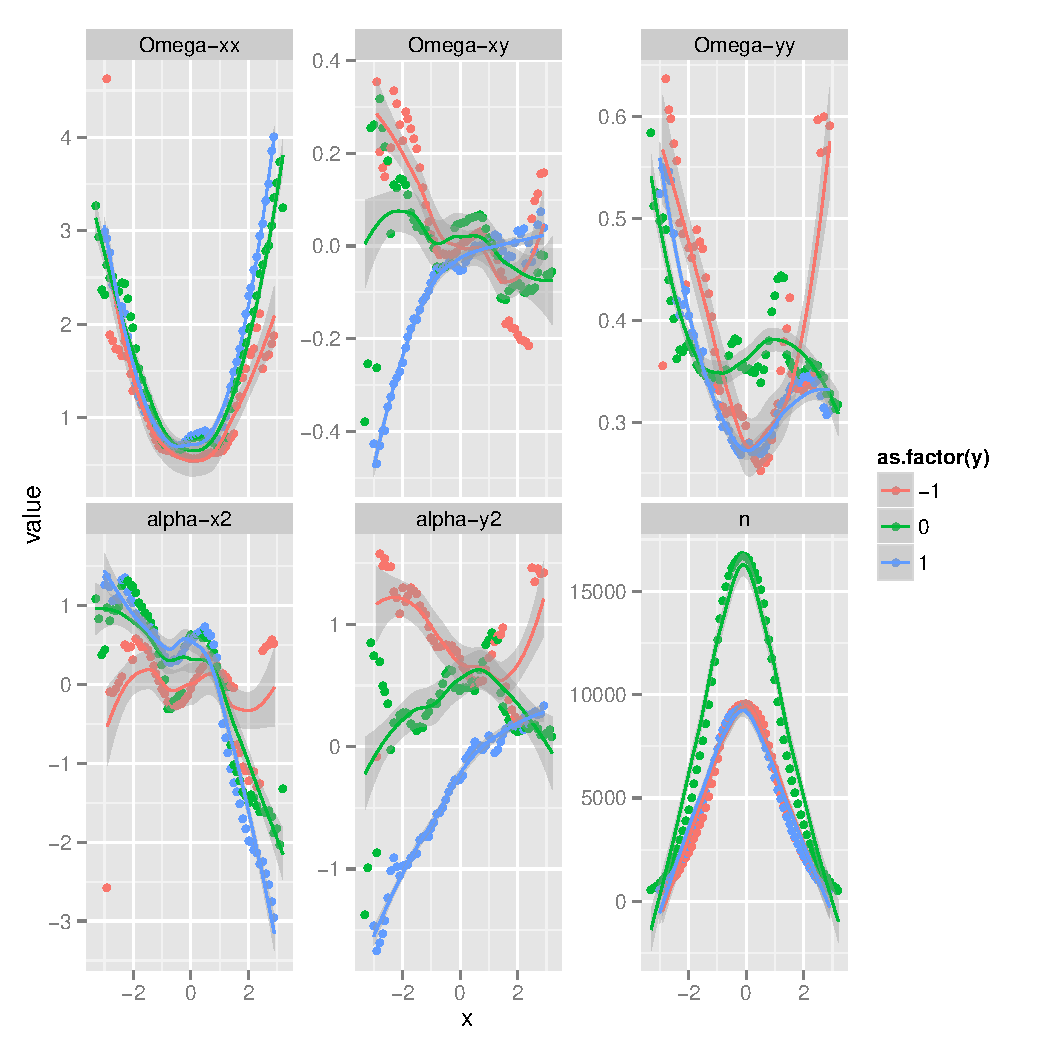
\includegraphics[width=13cm]{../scripts/flow/paramsChagingOverSpace.pdf}
\caption{Multivariate skew-normal parameters over space.}
\label{fig:smParamsOverSpace}
\end{figure}


\begin{table}
\centering

\begin{tabular}{c c}

parameter & equation \\
\hline
$\Omega_{x,x}$	& $= 0.33+ 0.38x^2 -0.29y^2 + 0.02x^4 + 0.22y^4$ \\ 
$\Omega_{x,y}$	& $=x + y + x^2 + y^2 + x^3 + y^3 + x^4 + y^4$ \\ 
$\Omega_{y,x}$	& $=x + y + x^2 + y^2 + x^3 + y^3 + x^4 + y^4$ \\ 
$\Omega_{y,y}$	& $=x + y + x^2 + y^2 + x^3 + y^3 + x^4 + y^4$ \\ 
\hline
$\alpha_{x^2}$		& $=x + y + x^2 + y^2 + x^3 + y^3 + x^4 + y^4$ \\ 
$\alpha_{y^2}$		& $=x + y + x^2 + y^2 + x^3 + y^3 + x^4 + y^4$ \\ 
\hline
$\nu$			& $=x + y + x^2 + y^2 + x^3 + y^3 + x^4 + y^4$ \\ 
\end{tabular}

\caption{Parameter model - clearly I still have to fill in all the coefficients!}
\label{tab:paramModel}
\end{table}

\subsubsection{Discussion}



\subsection{Coarse-to-fine}

People make shorter saccades over time. Include $1/f$ dynamics? 

\subsection{Left v Right}

Initially more fixations to the left half of the image \citep{nuthmann-matthias2014}.

\section{Using Biases for Better Analysis}

We will use the the central bias \citep{clarke-tatler2014} and \textit{saccadic flow} in some different contexts to see what biases can do for vision research. :p


\subsection{Attentional Landscapes}

Or do we call them hotspot maps?

\subsection{ROC Analysis}

Example of using our models rather than shuffle approaches.

\subsection{Flow and Coarse to fine}
To what extent does saccadic flow account for coarse-to-fine dynamics

\subsection{Inverse Yarbus}

Do these biases allow us to improve inverse yarbus performance?

\subsection{Salience}

Does salience explain the less likely saccades? 

\section{Discussion}

\section*{Acknowledgements}

Thanks to Adelchi Azzalini for advice on using the \texttt{sn} package for \texttt{R}. And mention grants. 

\bibliographystyle{plainnat}
\small
\bibliography{literature}
\end{document}